\makeatletter
\def\input@path{{../styles/}{../../styles/}{../../../styles/}{../}{../../}{../../../}}
\makeatother


\documentclass{ee102_pset}
% macros.tex - Course meta information
\renewcommand{\course}{EE 102}
\renewcommand{\coursetitle}{Signal Processing and Linear Systems}
\renewcommand{\instructor}{Ayush Pandey}
\renewcommand{\semester}{Fall}
\renewcommand{\year}{2025}
\renewcommand{\shorttitle}{Week 1: Introduction to Signals}
% Use \renewcommand to avoid 'already defined' errors

% The following packages can be found on http:\\www.ctan.org
% \usepackage{graphics} % for pdf, bitmapped graphics files
%\usepackage{epsfig} % for postscript graphics files
%\usepackage{mathptmx} % assumes new font selection scheme installed
%\usepackage{times} % assumes new font selection scheme installed
\usepackage{amsmath} % assumes amsmath package installed
\usepackage{amssymb,mathtools}  % assumes amsmath package installed
\usepackage{xcolor}
\usepackage{pgfplots,subcaption}
\usepackage[hidelinks]{hyperref}
\usepackage{verbatim}
\usepackage{graphicx}
\usepackage{listings}
\usepackage{fancyhdr}
% \usepackage{geometry}
\usepackage{siunitx}
\usepackage[most]{tcolorbox}
\usepackage{enumitem}
\usepackage{environ}
% -------- listings (Python) ----------
\lstdefinestyle{py}{
  language=Python,
  basicstyle=\ttfamily\small,
  keywordstyle=\color{blue!60!black}\bfseries,
  commentstyle=\color{green!40!black},
  stringstyle=\color{orange!60!black},
  showstringspaces=false,
  columns=fullflexible,
  frame=single,
  framerule=0.3pt,
  numbers=left,
  numberstyle=\tiny,
  xleftmargin=1em,
  tabsize=2,
  breaklines=true,
}

\usepackage[american]{circuitikz}
\usepackage{tikz}
\usetikzlibrary{arrows.meta,positioning,calc,angles,quotes}
\tikzset{
  >={Latex[length=2.2mm]},
  block/.style={draw, thick, rectangle, minimum height=10mm, minimum width=24mm, align=center},
  gain/.style={block, minimum width=14mm},
  sum/.style={draw, thick, circle, inner sep=0pt, minimum size=6mm},
  conn/.style={-Latex, thick},
}
\usepackage{caption}    
\usepackage{lscape}
\usepackage{soul}
\usepackage{physics}
\usepackage{hyperref}
\hypersetup{
    colorlinks=true,
    linkcolor=blue,
    filecolor=magenta,      
    urlcolor=blue,
    pdftitle={week1_notes},
    pdfpagemode=FullScreen,
}
%\usepackage{float} 

%\usepackage[demo]{graphicx}
\pgfplotsset{compat=1.18}
% \usepgfplotslibrary{fillbetween}

\newsavebox{\measurebox}

\let\proof\relax\let\endproof\relax


\def\abs#1{\left\lvert#1\right\rvert}
\let\proof\relax
\let\endproof\relax
\usepackage{amsthm}
\usepackage{accents}
\usepackage{relsize}
\newcommand{\ubar}[1]{\underaccent{\bar}{#1}}
\newtheorem{theorem}{Theorem}
\newtheorem{corollary}{Corollary}[theorem]
\newtheorem{lemma}{Lemma}
\newtheorem{proposition}{Proposition}
\newtheorem{statement}{Statement}

\theoremstyle{definition}
\newtheorem{definition}{Definition}
 
\theoremstyle{remark}
\newtheorem*{remark}{Remark}
\theoremstyle{remark}
\newtheorem*{claim}{Claim}
\setlength{\parindent}{0cm}
\newenvironment{nalign}{
    \begin{equation}
    \begin{aligned}
}{
    \end{aligned}
    \end{equation}
    \ignorespacesafterend
}


% Assignment info
\author{\rule{3cm}{0.4pt}} % Name placeholder
\submitdate{\rule{3cm}{0.4pt}} % Submission date placeholder
\problemset{Homework \#5: Applications of convolution and its properties}
\renewcommand{\duedate}{October 6, 2025}
\shorttitle{Homework \#5}

\begin{document}
\problem{1}
Consider the RC circuit discussed in class with input voltage $v_{\text{in}}(t)$ and output voltage measured across the capacitor $v_{\text{out}}(t)$. You may directly use the impulse response of this circuit for this problem.

Compute the convolution and graphically visualize (by hand, no programming) the output for the following inputs:

\problempart[20 points] A pulse input of amplitude $A$ lasting for $T$ seconds, starting at $t=0$:
\[
x(t) = \begin{cases}
A, & 0 \le t < T,\\
0, & \text{otherwise.}
\end{cases}
\]

\problempart[20 points] A sinusoidal voltage input of frequency $f$ Hz that is applied to the circuit after a delay of 5 seconds and taken away (set to 0 after 10 seconds):
\[
x(t) = A \sin(2 \pi f t) \left[u(t-5) - u(t-10)\right].
\]
\problem{2}
Prove that the convolution operation is associative. Although this holds true in both continuous-time and discrete-time, you should prove it for the discrete-time case only. Specifically, consider two systems with unit impulse responses: $h_1[n]$ and $h_2[n]$ given as:
\[
h_1[n] = \alpha^n u[n]
\]
for $\alpha = \tfrac{1}{4}$ and 
\[
h_2[n] = u[n-4] - 2u[n+1]
\]
for $n \in \mathbb{Z}$. The two systems are cascaded as shown in the block diagram below (Figure~\ref{fig:cascade}). 
\begin{figure}[h]
  \centering
  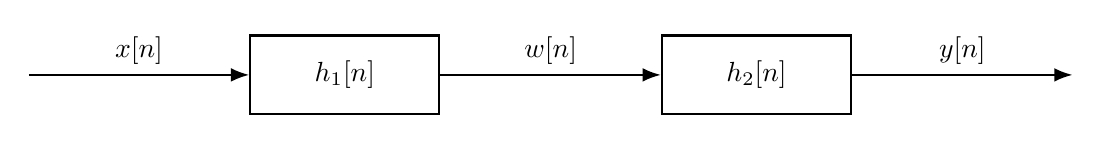
\begin{tikzpicture}
    % nodes
    \coordinate (in)  at (0,0);
    \node[block, right=2.8cm of in]   (Hone) {$h_1[n]$};
    \node[block, right=2.8cm of Hone] (Htwo) {$h_2[n]$};
    \coordinate[right=2.8cm of Htwo] (out);

    % arrows with labels
    \draw[conn] (in)  -- node[above] {$x[n]$} (Hone);
    \draw[conn] (Hone) -- node[above] {$w[n]$} (Htwo);
    \draw[conn] (Htwo) -- node[above] {$y[n]$} (out);
  \end{tikzpicture}
  \caption{Cascaded discrete-time LTI systems.}
  \label{fig:cascade}
\end{figure}

The final output $y[n]$ can be computed in two different ways:
\problempart [15 points] For the specific impulse responses given, compute $w[n] = x[n] * h_1[n]$ and then compute $y[n] = w[n] * h_2[n]$. That is, $y[n] = (x[n] * h_1[n]) * h_2[n]$. Obtain $y[n]$ in closed form.

\problempart [15 points] Alternatively, we can find $y[n]$ by first computing the overall impulse response of the cascaded system $h[n] = h_1[n] * h_2[n]$ and then convolving it with the input: $y[n] = x[n] * (h_1[n] * h_2[n])$. Obtain $y[n]$ in closed form.

\problempart [5 points] Show that the two results are equal, thus proving associativity of convolution. Write the associativity property of convolution (for three general signals) in your own words.

\problem{3}

Let $x[n]$ be a 1-D signal that represents grayscale colors as pixel intensities (0 is black and 255 is white):
\[
x[n] = [\,50,\;100,\;240,\;255,\;200,\;120,\;80,\;80,\;90,\;150,\;220,\;240\,],
\qquad 0\le n\le 11.
\]
Assume causal zero-padding outside the given range, that is, $x[n]=0$ for $n<0$ or $n>11$. Your goal is to compute $y[n]$ by hand and also using a for loop implementation (in Python or MATLAB) of the convolution sum. \textbf{You are not allowed to use external libraries to compute the convolution. Of course, you should use external libraries for plotting.}

{\color{red} Note: Helper code for plotting will be provided by Thursday night and this note will be updated.}

Consider the two physically meaningful impulse responses $h[\cdot]$ (both causal) of LTI systems:

\problempart A blurring system:
\[
h[n]=\tfrac13\,[\,\delta[n]+\delta[n-1]+\delta[n-2]\,]
\]

\problempart A first-difference (edge detector):
\[
h[n]=\delta[n]-\delta[n-1],
\]

For each of the parts above, 
\begin{enumerate}
  \item \textbf{4 points for each $h$} By hand, write the convolution sum for $y[n]$ and compute numerically $y[n]$ at $n=0,1,2$.
  \item \textbf{4 points for each $h$} Implement a for loop that computes $y[n]$ for all $n$ for system above. Make sure to plot the original $x[n]$ and each $y[n]$ on the same axes.
  \item \textbf{4 points for each $h$} Apply repeated convolution to intensify the effect of the system. You can choose one of the systems above and experiment with repeated convolutions.
\end{enumerate}

\problem{4}
\problempart [1 point] How long did this assignment take you to complete (this does not include the time spent in lectures or in labs, but it does include the time spent programming).
\end{document}
